\documentclass{article}
\usepackage{graphicx} % new way of doing eps files
\usepackage{listings} % nice code layout
\usepackage[usenames]{color} % color
\definecolor{listinggray}{gray}{0.9}
\definecolor{graphgray}{gray}{0.7}
\definecolor{ans}{rgb}{1,0,0}
\definecolor{blue}{rgb}{0,0,1}
% \Verilog{title}{label}{file}
\graphicspath{ {H:/ELC3338/Team8/CompOrg_Spring2018_S1_Team8/images/} }
\newcommand{\Verilog}[3]{
  \lstset{language=Verilog}
  \lstset{backgroundcolor=\color{listinggray},rulecolor=\color{blue}}
  \lstset{linewidth=\textwidth}
  \lstset{commentstyle=\textit, stringstyle=\upshape,showspaces=false}
  \lstset{frame=tb}
  \lstinputlisting[caption={#1},label={#2}]{#3}
}


\author{Matthew Carrano and Breana Leal}
\title{Lab 10 Memory}

\begin{document}
\maketitle

\section{Results}
The data memory and iMemory modules work correctly. Both modules were verified through the iMemory testbench which consisted of six tests, each a cycle long. Inside the test bench, the input variables are mem\_read, mem\_write, zero, branch, uncond\_branch, alu\_result, and read\_data2. All variable names correspond to the name in the datapath picture. The output variables are or\_result (the branch decision) and read\_data. read\_data corresponds to the picture, and or\_result is simply the result of the OR gate in the iMemory module. The goal of the first test was to verify the memory read capability as well as the or\_result when all branch related inputs are 0. It is seen from the simulation in Figure~\ref{fig:iMemorysim} on page~\pageref{fig:iMemorysim} that on the first positive edge of the clock, or\_result is 0 and read\_data is 1. This is expected because zero, branch, and uncond\_branch are all set to 0 which means the inputs of the OR gate are 0. Additionally, mem\_read is set to 1 and alu\_result to 2. This means the module should read the data from address 1 of data memory, and output that data through read\_data. Data memory was initialized with Figure~\ref{fig:ramData} on page~\pageref{fig:ramData}. Therefore, address 1 of data memory contains the value 1. This is why read\_data equals 1. On the two next cycles, the memory write functionality was tested. This was done by turning mem\_read off and mem\_read on, and then vice versa in the following cycle. alu\_result was also changed to 2 during the write test. In this way, the value of read\_data2, arbitrarily set to 1234 in the first cycle, is written to address 2 of data memory and in the next cycle (mem\_read = 1, mem\_write = 0) the value of address 2 is read from data memory. Therefore, alu\_data is 1234 at the start of the third cycle, as seen in the simulation. Finally, the branch decision was tested further. First, branch was set to 1, while the other branch-related inputs remained at zero. With the zero flag set to 0, the AND gate will output 0, and therefore both inputs of the OR gate are zero. Therefore, the or\_result is 0. Next, zero was set to 1. This means the AND gate will output 1, and therefore the or\_result is 1. Lastly, branch and zero are set to 0, but uncond\_branch to 1. Thus, one of the OR gate inputs is 1 and so its output is also 1. 

\begin{figure}[t]	
	\caption{Data Memory initial values.}
	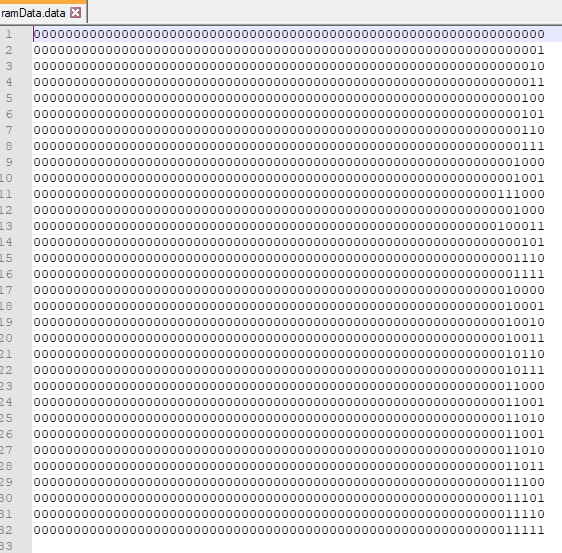
\includegraphics[scale=0.75]{ramData}
	\label{fig:ramData}
\end{figure}
\clearpage

\section{Code}

\Verilog{Verilog code for implementing the data\_memory module.}{code:data_memory}{../code/4_memory/data_memory.v}
\Verilog{Verilog code for implementing the iMemory module.}{code:iMemory}{../code/4_memory/iMemory.v}
\Verilog{Verilog code for implementing the iMemory Testbench.}{code:iMemory Testbench}{../code/4_memory/iMemory_test.v}


\section{Simulation}

\begin{figure}[h]	
	\caption{Timing diagram for iMemory module test. All values are in decimal.}
	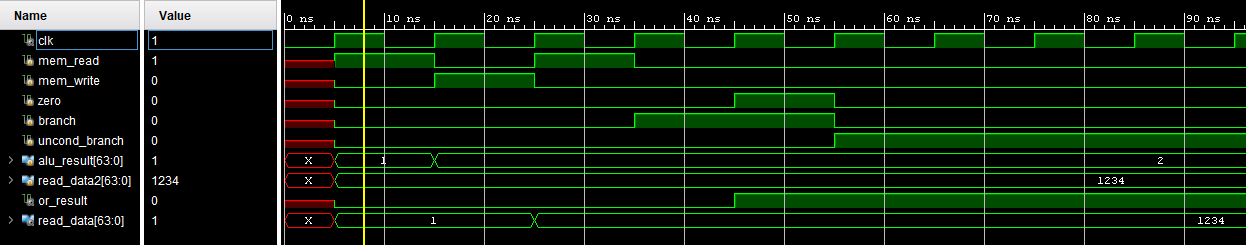
\includegraphics[width=\textwidth]{iMemory_sim}
	\label{fig:iMemorysim}
\end{figure}


\end{document} 